\lecdate{24.10.2017}
\sectionN{Formales statisches Neuronenmodell}
$$\vec{x} = \begin{pmatrix}
x_1 \\ x_2 \\ \vdots \\ x_n
\end{pmatrix}
\To
\vec{w}_i=
\begin{pmatrix}
w_{1i}\\
w_{2i}\\
\vdots\\
w_{ni}
\end{pmatrix}
$$

$z_i=f(\vec{x}, \vec{w}_i$ … Zustand des Neurons $i$\\
$y_i=f(z_i)$ … Ausgabe des Neurons $i$

\subsectionN{Zustandsfunktionen}
\begin{anumerate}
\item auf Basis des Skalarprodukts\\
$z_i = w_{1i} \cdot x_1 + w_{2i}\cdot x_2 + \ldots + w_{ni}\cdot x_n - \Theta_i$\quad($\Theta_i$: Schwellwert)
\item auf Basis von Abstandsfunktionen\\
z.B. $z_i=\sqrt{(x_1-w_{1i})^2+\ldots+(x_n-w_{ni})^2}= L_2\text{-Norm bzw. euklidischer Abstand}$\\
Norm: $L_m=\sqrt[n]{(x_1-w_{1i})^m+\ldots+(x_n-w_{ni})^m}$\\
($L_1$-Norm wäre City-Block-Distanz)
\end{anumerate}

\subsectionN{Ausgabe- bzw. Transferfunktion}
\begin{enumerate}[label=(\arabic*)]
\item $y_i = f(z_i) = \frac{1}{1+e^{-z_i}}\To$ Fermi-  bzw. Signoidfunktion
\begin{center}
\begin{tikzpicture}
\begin{axis}[hide axis, axis equal, clip=false, scale=.5]
\addplot[domain=-2:2] {1/(1+e^(-4*x))}; 
\draw [-latex](-2.5,0) -- (2.5,0) node[below left]{$z_s$};
\draw [-latex](0,-0.1) -- (0,1.5) node[above right]{$y_s$}; 
\draw (0.1,1) -- (-0.1,1) node[left]{$1$};
\end{axis}
\end{tikzpicture}
\end{center}
\item $y_i = f(z_i)= \mathrm{sgn}(z_i) = \begin{cases}
0 & \text{für }z_i \leq 0\\
1 & \text{für }z_i >0
\end{cases}$
\item $y_i = f(z_i) = \exp \left( -\frac{z_i^2}{2 \sigma_i^2}\right)$
\begin{center}
\begin{tikzpicture}
\begin{axis}[hide axis, axis equal, clip=false, scale=.5]
\addplot[domain=0:3] {e^(-x^2/2)};
\draw [-latex](-0.5,0) -- (3.5,0) node[below left]{$z_i$};
\draw [-latex](0,-0.1) -- (0,2) node[above right]{$y_i$}; 
\draw (0.1,1) -- (-0.1,1) node[left]{$1$};
\draw [-latex] (0,0.5) -- (1,0.5) node [below left]{$\sigma_i$};
\end{axis}
\end{tikzpicture}
\end{center}
\end{enumerate}
Funktionen (1) und (2) setzen Skalarproduktaktivierfunktion voraus, Funktion (3) eine distanz-basierte Zustandsberechunng.

\subsectionN{Beispiel Skalarproduktaktivierfunktion}
Welche Funktion kann nur \underline{ein} Neuron mit Skalarproduktaktivierfunktion realisieren?
\begin{center}
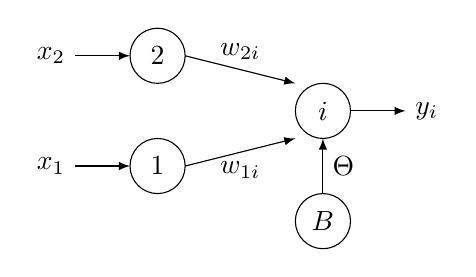
\begin{tikzpicture}[scale=.7]
\draw  (0,0) circle (0.5) node{$2$};
\draw  (0,-2) circle (0.5) node{$1$};
\draw [-latex](-1.5,0) node[left]{$x_2$} -- (-0.5,0);
\draw [-latex](-1.5,-2) node[left]{$x_1$} -- (-0.5,-2);
\draw  (3,-1) circle (0.5) node{$i$};
\draw [-latex](0.5,0) -- node[above]{$w_{2i}$} (2.5,-0.5);
\draw [-latex](0.5,-2) -- node[below]{$w_{1i}$} (2.5,-1.5);
\draw [-latex](3.5,-1) -- (4.5,-1) node[right]{$y_i$};
\draw  (3,-3) circle (0.5) node{$B$};
\draw [-latex](3,-2.5) -- node[right]{$\Theta$} (3,-1.5);
\end{tikzpicture}\\
$B$: Bias-Neuron mit konstanter Ausgabe von $1$.
\end{center}
$$z_i=w_{1i}\cdot x_i + w_{2i}x_2-\Theta_i$$
$$y_i = f(z_i) = z_i$$
Beispieldaten (AND-Abbildung):
\begin{center}
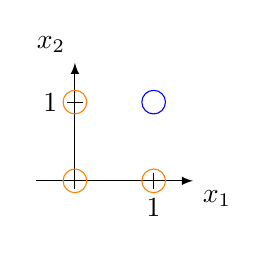
\begin{tikzpicture}
\draw [-latex](-0.5,0) -- (1.5,0) node[below right]{$x_1$};
\draw [-latex](0,-0.1) -- (0,1.5) node[above left]{$x_2$}; 
\draw (0.1,1) -- (-0.1,1) node[left]{$1$};
\draw (1,0.1) -- (1,-0.1) node[below]{$1$};

\draw [orange] (0,1) circle (0.15);
\draw [orange] (0,0) circle (0.15);
\draw [orange] (1,0) circle (0.15);
\draw [blue] (1,1) circle (0.15);
\end{tikzpicture}
\end{center}
Neuron $i$ soll für $\vec{x}=(1,1)^T$ eine Ausgabe $>0$ und für $\vec{x}=(0,0)^T,\;(0,1)^T\;(1,0)^T$ Ausgabe $\geq 0$ liefern.\bigskip

Setze die Parameter $w_{1i}, \; w_{2i}$ und $\Theta_i$ so, dass die gewünschte Funktion entsteht:

z.B.: $w_{1i}=w_{2i}=1$; $\Theta=1$\\
Probe:\\
$\vec{x}^1=(0,0)^T$: $z_i=1\cdot 0 + 1 \cdot 0 -1 = -1\; \checkmark$\\
$\vec{x}^2=(0,1)^T$: $z_i=1\cdot 1 + 1 \cdot 0 -1 = \phantom{-}0\; \checkmark$\\
$\vec{x}^3=(1,0)^T$: $z_i=1\cdot 0 + 1 \cdot 1 -1 = \phantom{-}0\; \checkmark$\\
$\vec{x}^4=(1,1)^T$: $z_i=1\cdot 1 + 1 \cdot 1 -1 = \phantom{-}1\; \checkmark$\bigskip

Neuron bildet eine Lineare Diskriminanzfunktion aus ($\RR^2\To$Gerade, $\RR^2\To$Ebene, $\RR^n\To$ Hyperebene), die den Eingaberaum in zwei Hälften teilt.
\begin{center}
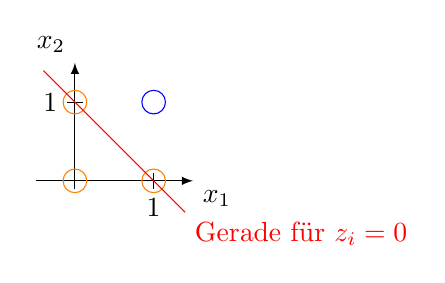
\begin{tikzpicture}
\draw [-latex](-0.5,0) -- (1.5,0) node[below right]{$x_1$};
\draw [-latex](0,-0.1) -- (0,1.5) node[above left]{$x_2$}; 
\draw (0.1,1) -- (-0.1,1) node[left]{$1$};
\draw (1,0.1) -- (1,-0.1) node[below]{$1$};

\draw [orange] (0,1) circle (0.15);
\draw [orange] (0,0) circle (0.15);
\draw [orange] (1,0) circle (0.15);
\draw [blue] (1,1) circle (0.15);
\draw [red](-0.4,1.4) -- (1.4,-0.4) node[below right]{Gerade für $z_i=0$};
\end{tikzpicture}
\end{center}
$\to$ Neuron realisiert eine Halbraumtrennung.\\
mit $y_i=\frac{1}{1+e^{-z_i}}$: 
\begin{center}
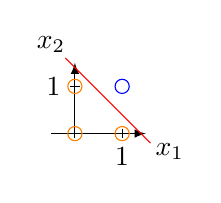
\begin{tikzpicture}[scale=.6]
\draw [-latex](-0.5,0) -- (1.5,0) node[below right]{$x_1$};
\draw [-latex](0,-0.1) -- (0,1.5) node[above left]{$x_2$}; 
\draw (0.1,1) -- (-0.1,1) node[left]{$1$};
\draw (1,0.1) -- (1,-0.1) node[below]{$1$};

\draw [orange] (0,1) circle (0.15);
\draw [orange] (0,0) circle (0.15);
\draw [orange] (1,0) circle (0.15);
\draw [blue] (1,1) circle (0.15);
\draw [red](-0.2,1.6) -- (1.6,-0.2);
\end{tikzpicture}
\end{center}

Offset/Schwelle ($\Theta$) gibt Abstand zum Ursprung an.

\subsectionN{Ermittlung optimale Parameter}
Wie ermittelt lineares Neuron sein optimalen Parameter?

Ausgangspunkt sei Hebb'sche Lernregel:
\begin{center}
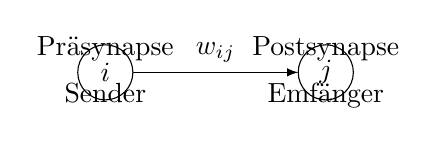
\begin{tikzpicture}[scale=.7]
\draw (0,0) circle (0.5) node{$i$} node[above=.5]{Präsynapse}  node[below=.5]{Sender};
\draw (4,0) circle (0.5) node{$j$} node[above=.5]{Postsynapse}  node[below=.5]{Emfänger};
\draw [-latex] (0.5,0) -- node[above]{$w_{ij}$}(3.5,0);
\end{tikzpicture}
\end{center}
$$\Delta w_{ij} = \eta \cdot y_i \cdot y_j \quad \eta\text{: Lernrate}$$
Wir erweitern diese Lernregel und ersetzen den postsynaptischen Term $y_j$ durch einen \emph{Fehlerterm}!\\
Wir kennen zu jedem Eingabevektor die gewünschte Ausgabe (Zielausgabe bzw. \torange{Teachvorgabe}).\\
Am Bsp. der AND-Abbildung:\\
\begin{tabular}{c c | c}
$x_1$ & $x_2$ & \torange{$t$}\\\hline
0 & 0 & 0\\
0 & 1 & 0\\
1 & 0 & 0\\
1 & 1 & 1
\end{tabular}\\
Fehlerterm:\\
$(t-y_j)$ $\To$ Differenz zwischen tatsächlicher Ausgabe $y_j$ und gewünschter Ausgabe $t$.\\
Lernregel lautet jetzt:
$$\boxed{\Delta w_{ij}=\eta \cdot y_i \cdot (t-y_j)}$$
$\to$ \emph{Delta-Lernregel} bzw. \emph{Perceptron-Lernregel}\\
$(t-y_j)$: Fehler auf Ausgabeseite
\begin{center}
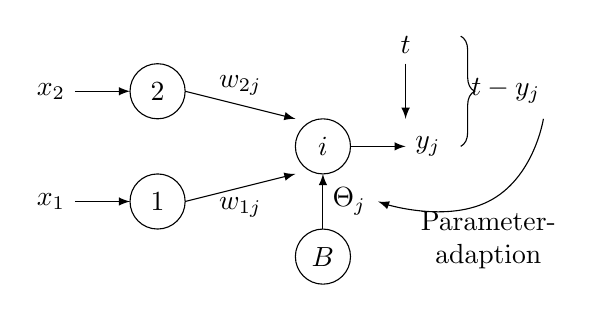
\begin{tikzpicture}[scale=.7]
\draw  (0,0) circle (0.5) node{$2$};
\draw  (0,-2) circle (0.5) node{$1$};
\draw [-latex](-1.5,0) node[left]{$x_2$} -- (-0.5,0);
\draw [-latex](-1.5,-2) node[left]{$x_1$} -- (-0.5,-2);
\draw  (3,-1) circle (0.5) node{$i$};
\draw [-latex](0.5,0) -- node[above]{$w_{2j}$} (2.5,-0.5);
\draw [-latex](0.5,-2) -- node[below]{$w_{1j}$} (2.5,-1.5);
\draw [-latex](3.5,-1) -- (4.5,-1) node[right]{$y_j$};
\draw  (3,-3) circle (0.5) node{$B$};
\draw [-latex](3,-2.5) -- node[right]{$\Theta_j$} (3,-1.5);
\draw [-latex](4.5,0.5) node[above]{$t$} -- (4.5,-0.5);
\draw [decorate, decoration={brace, amplitude=5pt}](5.5,1) -- node[right=.3]{$t-y_j$} (5.5,-1);
\draw [-latex] plot[smooth, tension=1] coordinates {(7,-0.5) (6,-2) (4,-2)};
\node at (6,-2)[below = .2, align=center]{Parameter-\\adaption};
\end{tikzpicture}
\end{center}
Mit dieser Lernregel durchläuft man den Trainingsdatensatz so lange, bis die Differenz zwischen $t$ und $y_i$ für alle Trainingsbeispiele minimal ist.

Diese Lernregel bildet die Basis für das Perceptron-Netzwerk (60er Jahre). Dies ist ein einschichtiges Netzwerk aus Sklarproduktneuronen: Beliebig viele $x_n$ werden von beliebig vielen $j_m$ verarbeitet.

Wie muss man sowohl das Netzwerk als auch die Lernregel erweitern, damit beliebig geformte Regionen voneinander separiert werden können?\\
$\To$ vom Perceptron zum Multi-Layer-Perceptron (MLP)\bigskip

\subsectionN{Beispiel XOR}
Bei Belegungen mit Anordnungen wie beim XOR:
\begin{center}
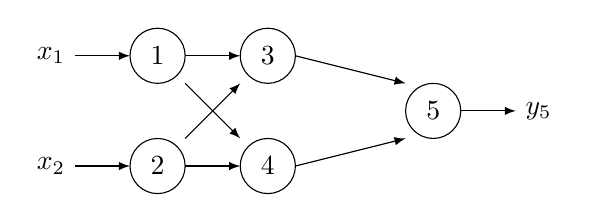
\begin{tikzpicture}[scale=.7]
\draw  (-2,0) circle (0.5) node{$1$};
\draw  (-2,-2) circle (0.5) node{$2$};
\draw [-latex](-3.5,0) node[left]{$x_1$} -- (-2.5,0);
\draw [-latex](-3.5,-2) node[left]{$x_2$} -- (-2.5,-2);
\draw  (0,0) circle (0.5) node{$3$};
\draw  (0,-2) circle (0.5) node{$4$};
\draw [-latex](-1.5,0)-- (-0.5,0);
\draw [-latex](-1.5,-2)-- (-0.5,-2);
\draw  (3,-1) circle (0.5) node{$5$};
\draw [-latex](0.5,0) -- (2.5,-0.5);
\draw [-latex](0.5,-2) -- (2.5,-1.5);
\draw [-latex](3.5,-1) -- (4.5,-1) node[right]{$y_5$};
\draw [-latex](-1.5,-1.5) -- (-0.5,-0.5);
\draw [-latex](-1.5,-0.5) -- (-0.5,-1.5);
\end{tikzpicture}
\end{center}
Neuronen 1, …, 5 sind Skalarprodukt-neuronen mit $y_i = \frac{1}{1+e^{-z_i}}$ $\to$ stetig differenzierbare Funktion. Für unsere Darstellung der $y_4$-$y_5$-Ebene verwenden wir $y=f(z) = \begin{cases}
1 & \text{für } z> 0\\
0 & \text{für }z \leq 0
\end{cases}$

Wertetabelle:\\
\begin{tabular}{c c | c}
$x_1$ & $x_2$ & t\\\hline
0 & 0 & 0\\
0 & 8 & 1\\
8 & 0 & 1\\
8 & 8 & 0\\
\end{tabular}
\begin{center}
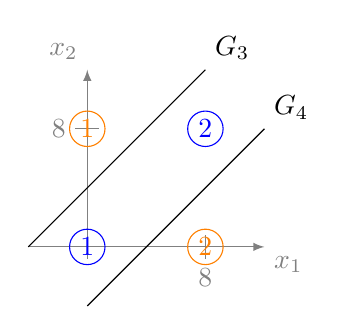
\begin{tikzpicture}[scale=1.5]
\draw [-latex, gray](-0.5,0) -- (1.5,0) node[below right]{$x_1$};
\draw [-latex, gray](0,-0.1) -- (0,1.5) node[above left]{$x_2$}; 
\draw [gray](0.1,1) -- (-0.1,1) node[left]{$8$};
\draw [gray](1,0.1) -- (1,-0.1) node[below]{$8$};

\draw [orange] (0,1) circle (0.15) node{$1$};
\draw [blue] (0,0) circle (0.15) node{$1$};
\draw [orange] (1,0) circle (0.15) node{$2$};
\draw [blue] (1,1) circle (0.15) node{$2$};
\draw (-0.5,0) -- (1,1.5) node[above right]{$G_3$};
\draw (0,-0.5) -- (1.5,1) node[above right]{$G_4$};
\end{tikzpicture}
\end{center}
Graphisches Ablesen/Ausrechnen der Parameter für Neuronen 3 und 4 liefert bspw.:\\
$w_{13}=1$; $w_{23}=-1$; $\Theta_3=-3$\\
$w_{14}=1$; $w_{24}=-1$; $\Theta_4=3$\\
$(0,0)^T$: $z_3=w_{13}x_1+w_{23}x_2-\Theta_3=3$; $y_3=1$, $z_4=w_{14}\ldots-\Theta_4=-3$; $y_4=0$\\
$(0,8)^T$: $z_3=-5 \to y_3=0$, $z_4=-11 \to y_4 = 0$\\
$(8,0)^T$: $z_4=12 \to y_3=1$, $z_4=5 \to y_4=1$\\
$(8,8)^T$: $z_3=3 \to y_3=1$, $z_4=-3 \to y_4 = 0$
\begin{center}
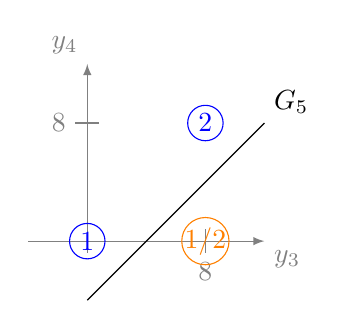
\begin{tikzpicture}[scale=1.5]
\draw [-latex, gray](-0.5,0) -- (1.5,0) node[below right]{$y_3$};
\draw [-latex, gray](0,-0.1) -- (0,1.5) node[above left]{$y_4$}; 
\draw [gray](0.1,1) -- (-0.1,1) node[left]{$8$};
\draw [gray](1,0.1) -- (1,-0.1) node[below]{$8$};
\draw [blue] (0,0) circle (0.15) node{$1$};
\draw [orange] (1,0) circle (0.2) node{$1/2$};
\draw [blue] (1,1) circle (0.15) node{$2$};
\draw (0,-0.5) -- (1.5,1) node[above right]{$G_5$};
\end{tikzpicture}
\end{center}

\sectionN{Delta Lernregel}
\lecdate{07.11.2017}
$$\Delta w_{ij} = \eta \cdot y_i \cdot (t_j - y_j)$$
$\To$ gültig für \emph{Perceptoren}.\\
Ziel: Lernregel finden, mit der Parameter eines mehrschichtigen Netzwerks adaptiert werden können.
\subsection{Mehrschichtiges Netzwerk}
$\to$ \emph{Multilayer-Perceptron} (MLP)





